\documentclass[10pt, a4paper]{article}
\usepackage[top=3cm, bottom=4cm, left=3.5cm, right=3.5cm]{geometry}
\usepackage{amsmath,amsthm,amsfonts,amssymb,amscd, fancyhdr, color, comment, graphicx, environ}
\usepackage{float}
\usepackage{mathtools}
\usepackage{mathrsfs}
\usepackage[math-style=ISO]{unicode-math}
\DeclareSymbolFont{\mathnormal}{letters}
\usepackage{lastpage}

%%%%%%%%%%%%%%%%%%%%%%%%%%%%%%%%%%%%%%%%%%%%%%%%%%%%%%%%%%%%%%%%%%
%%%%%%%%%%%%%%%%%%%%%%%%%%%%%%%%%%%%%%%%%%%%%%%%%%%%%%%%%%%%%%%%%%
%Fill in the appropriate information below
\newcommand{\norm}[1]{\left\lVert#1\right\rVert}     
\newcommand\course{ECON 8010}                            % <-- course name   
\newcommand\hwnumber{6}                                  % <-- homework number
\newcommand\Information{Tate Mason}                        % <-- personal information
%%%%%%%%%%%%%%%%%%%%%%%%%%%%%%%%%%%%%%%%%%%%%%%%%%%%%%%%%%%%%%%%%%
%%%%%%%%%%%%%%%%%%%%%%%%%%%%%%%%%%%%%%%%%%%%%%%%%%%%%%%%%%%%%%%%%%
%Page setup
\pagestyle{fancy}
\headheight 35pt
\lhead{\today}
\rhead{}
\lfoot{}
\pagenumbering{arabic}
\cfoot{\small\thepage}
\rfoot{}
\headsep 1.2em
\renewcommand{\baselinestretch}{1.25}
%%%%%%%%%%%%%%%%%%%%%%%%%%%%%%%%%%%%%%%%%%%%%%%%%%%%%%%%%%%%%%%%%%
%%%%%%%%%%%%%%%%%%%%%%%%%%%%%%%%%%%%%%%%%%%%%%%%%%%%%%%%%%%%%%%%%%
%Add new commands here
\renewcommand{\labelenumi}{\alph{enumi})}
\newcommand{\var}{\text{var}}
\newcommand{\Z}{\mathbb Z}
\newcommand{\R}{\mathbb R}
\newcommand{\Q}{\mathbb Q}
\newcommand{\NN}{\mathbb N}
\newcommand{\PP}{\mathbb P}
\DeclareMathOperator{\Mod}{Mod} 
\renewcommand\lstlistingname{Algorithm}
\renewcommand\lstlistlistingname{Algorithms}
\def\lstlistingautorefname{Alg.}
\newtheorem*{theorem}{Theorem}
\newtheorem*{lemma}{Lemma}
\newtheorem{case}{Case}
\newcommand{\assign}{:=}
\newcommand{\infixiff}{\text{ iff }}
\newcommand{\nobracket}{}
\newcommand{\backassign}{=:}
\newcommand{\tmmathbf}[1]{\ensuremath{\boldsymbol{#1}}}
\newcommand{\tmop}[1]{\ensuremath{\operatorname{#1}}}
\newcommand{\tmtextbf}[1]{\text{{\bfseries{#1}}}}
\newcommand{\tmtextit}[1]{\text{{\itshape{#1}}}}

\newenvironment{itemizedot}{\begin{itemize} \renewcommand{\labelitemi}{$\bullet$}\renewcommand{\labelitemii}{$\bullet$}\renewcommand{\labelitemiii}{$\bullet$}\renewcommand{\labelitemiv}{$\bullet$}}{\end{itemize}}
\catcode`\<=\active \def<{
\fontencoding{T1}\selectfont\symbol{60}\fontencoding{\encodingdefault}}
\catcode`\>=\active \def>{
\fontencoding{T1}\selectfont\symbol{62}\fontencoding{\encodingdefault}}
\catcode`\<=\active \def<{
\fontencoding{T1}\selectfont\symbol{60}\fontencoding{\encodingdefault}}

%%%%%%%%%%%%%%%%%%%%%%%%%%%%%%%%%%%%%%%%%%%%%%%%%%%%%%%%%%%%%%%%%%
%%%%%%%%%%%%%%%%%%%%%%%%%%%%%%%%%%%%%%%%%%%%%%%%%%%%%%%%%%%%%%%%%%
%Begin now!

\begin{document}
  \begin{titlepage}
    \begin{center}
      \vspace*{3cm}
            
        \vspace{1cm}
        \huge
        Homework \hwnumber
            
        \vspace{1.5cm}
        \Large
            
        \textbf{\Information}                      % <-- author
            
        \vfill
        
        A \course \ Homework Assignment
            
        \vspace{1cm}
        \Large

        
        \today
            
    \end{center}
  \end{titlepage}

  \newpage
\section*{Problem 1. Sandholm PS2 \# 7}
  Two players choose actions from the unit interval. Player $i$'s von-Neumann Morgenstern utility, expressed as a function of his action $x_i\in[0,1]$ and his opponent's action $x_j\in[0,1]$, is 
    \begin{gather*}
      u_i(x_i,x_j) = \begin{cases}
        (\theta_i+3x_j-4x_i)x_i \ if \ x_j<\frac{2}{3}\\
        (3x_j-2)x_i \ if \ x_j\geq\frac{2}{3}
      \end{cases}
    \end{gather*}
    Find all pure Nash equilibria of the normal form game $G$ in which $\theta_1=\theta_2=2$ 
  \subsection*{Solution}
    Case 1:
    \begin{gather*}
      \frac{\partial u}{\partial x_i} = 2 + 3x_j - 8x_i = 0 \rightarrow x_i = \frac{2+3x_j}{8} \\
      0 \leq \frac{2+3x_j}{8} \leq 1 \rightarrow -\frac{2}{3} \leq x_j \leq 2\\
    \end{gather*}
    By symmetry, given both maximize and have complete info, $x_i=x_j=\frac{2}{5}$

    Case 2:
    Both players would maximize, choosing $x_i=x_j=1$. This is due to the fact that they will choose the highest possible value from the interval available to them.
\section*{Problem 2. Sandholm PS3 \# 4}
  (i) Find all subgame perfect equilibria of the game in Figure 1 below.
  (ii) Determine the reduced normal form of this game. 
  \begin{center}
    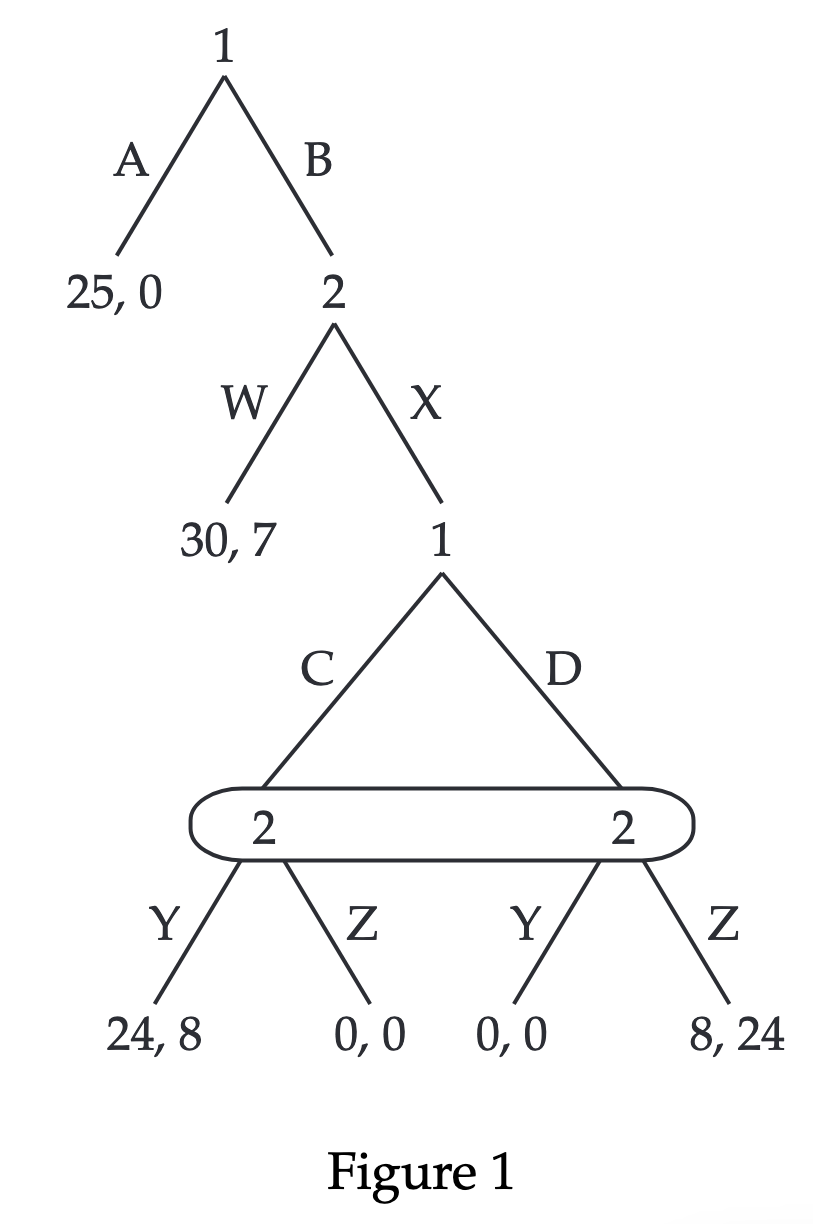
\includegraphics[width = 0.25\textwidth]{fig1.png}
  \end{center}
  \subsection*{Solution}
    \subsubsection*{(i)}
      There is one pure subgame equilibrium in which player 1 chooses A every time, leaving the rest of the moves irrelevant and thus player 2 is indifferent.
      \begin{gather*}
        ((A,C),(X,Y))
      \end{gather*}
      Further, there is a mixed strategy in which Player 2 will play W, thus drawing Player 1 to play B
      \begin{gather*}
        \EE(Y) = 8, \EE(Z) = 24 \\
        8Y = 24Z \rightarrow Y = 3Z \\
        Y + Z = 1 \rightarrow 3Z + Z = 1 \Rightarrow Z = \frac{1}{4} \\ 
        \therefore Y = \frac{3}{4} \\
        ((B, \beta C + (1-\beta)D), (W, \frac{3}{4}Y + \frac{1}{4}Z))
      \end{gather*}
      Finally, there is an equilibrium in which everyone is indifferent.
      \begin{gather*}
        ((\alpha A + (1-\alpha)B, \beta C + (1-\beta)D),(\frac{5}{6}W + \frac{1}{6}X,\frac{3}{4}Y+\frac{1}{4}Z))
      \end{gather*}
    \subsubsection*{(ii)}
      \begin{center}
        \begin{tabular}{|c|c|c|c|c|}
            \hline
          & WY & WZ & XY & XZ \\
          \hline
          A & 25,0 & 25,0 & 25,0 & 25,0 \\
          \hline
          BC & 30,7 & 30,7 & 24,8 & 0,0 \\
          \hline
          BD & 30,7 & 30,7 & 0,0 & 8,24 \\
          \hline
        \end{tabular}
      \end{center}
\section*{Problem 3. Sandholm PS3 \# 7}
  Arthur and Beatrix compete in a race. At the start of the race, both players are 6 steps away from the finish line. Who gets the first turn is determined by a toss of a fair coin; the players then alternate turns, with the results of all previous turns being observed before the current turn occurs.
  During a turn, a player chooses from these four options:
  \begin{enumerate}
    \item Do nothing at cost 0;
    \item Advance 1 step at cost 2;
    \item Advance 2 steps at cost 7;
    \item Advance 3 steps of at cost 15.
  \end{enumerate}
  The race ends when the first player crosses the finish line. The winner of the race receives a payoff of 20, while the loser gets nothing. Finally, there is discounting: after each turn, payoffs are discounted by a factor of $\delta$, where $\delta$ is less than but very close to 1.
  \subsubsection*{(i)}
  Find all subgame perfect equilibria of this game. (Hint: In all subgame perfect equilibria, a player's choice at a decision node only depends on the number of steps he has left and on the number of steps his opponent has left. To help take advantage of this you might want to write down a table.)
  \subsubsection*{(ii)} 
  Suppose that Arthur wins the coin toss. Compare his equilibrium behavior with his optimal behavior in the absence of competition. Provide intuition for any similarities or differences you find.
  \subsection*{Solution}
    \subsubsection*{(i)}
      \begin{center}
        \begin{tabular}{|c|c|c|c|c|c|c|}
          \hline
          & 1 & 2 & 3 & 4 & 5 & 6 \\
          \hline
          1 & A1 & A1 & A1 & A1 & A1 & A1 \\
          2 & A1 & A1 & A1 & A1 & A1 & A1 \\
          3 & A1 & A1 & A1 & A1 & A1 & A1 \\
          4 & A0 & A0 & A0 & A1 & A1 & A1 \\
          5 & A0 & A0 & A0 & A0 & A1 & A1 \\
          6 & A0 & A0 & A0 & A0 & A1 & A2 \\
          \hline
        \end{tabular}
      \end{center}
    The game exhibits first mover advantage. Thus the optimal path is to move as quickly as possible for both players. Player 1 will move 2, with player 2 choosing not to move since they are unable to win. Thus, player 1 will then only move in single step increments, minimizing cost. This leads to player 1 spending 15 and player 2 spending 0. 
  \subsubsection*{(ii)}
    In the absence of competition, the need to move 3 at the start is eliminated, thus the player will move 1 step at a time, minimizing cost.
  \begin{center}
    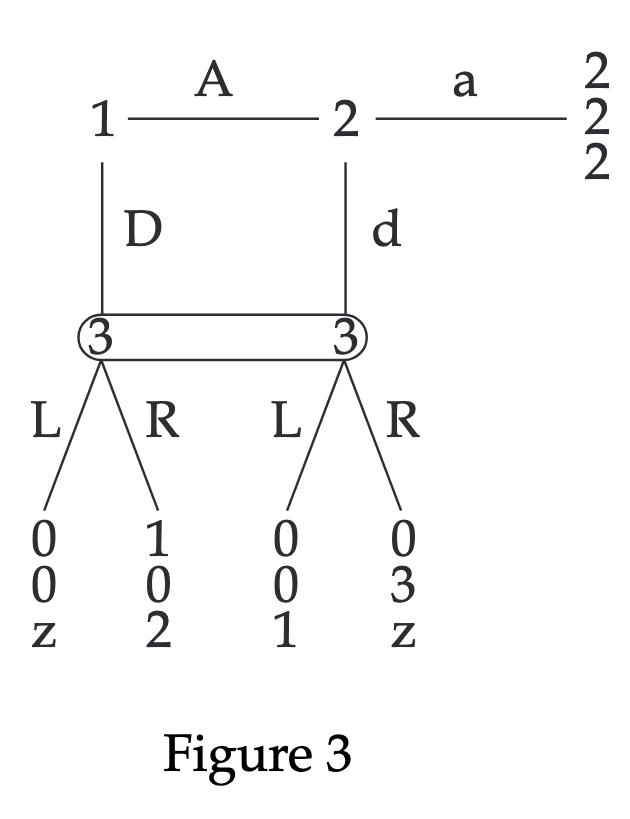
\includegraphics[width=0.25\textwidth]{fig3.png}
  \end{center}
\section*{Problem 4. Sandholm PS4 \# 1}
  Compute all sequential equilibria of the game in Figure 3 when $z=3$.
  \subsection*{Solution}
    The sequential equilibrium when $z=3$ is 
    \begin{gather*}
      (A, \frac{1}{3}a + \frac{2}{3}d, \frac{1}{3}L + \frac{2}{3}R).
    \end{gather*}
    I am still working to learn the notation, so I will use words. When solving for player 3's best response, it is found that playing L one-third of the time and R two-thirds is optimal for them. Then, when using that information for player 2, it sis found that they will receive a higher payoff when playing d than a given the strategy for player 3. Finally, player 1 is best off playing A in all cases since it gives them a higher payoff than if they were to play D.  
\section*{Problem 5. Sandholm PS4 \# 2}
  Compute all sequential equilibria of the game in Figure 3 when $z=2$.
  \subsection*{Solution}
    The sequential equilibrium when $z=2$ is 
    \begin{gather*}
      (A,a,R)
    \end{gather*}
    When z=2, Players 1 and 2 will play to get the guaranteed payoff, rather than leaving to player 3 who will play R every time given the available moves.
\section*{Problem 6. Sandholm PS4 \# 3}
  For the game in Figure 4 below, specify an assessment (i.e., a strategy profile and a belief profile) with these three properties: (i) beliefs are Bayesian; (ii) no player has a profitable one-shot deviation at any information set; (iii) the assessment is not a weak sequential equilibrium.
  \begin{center}
    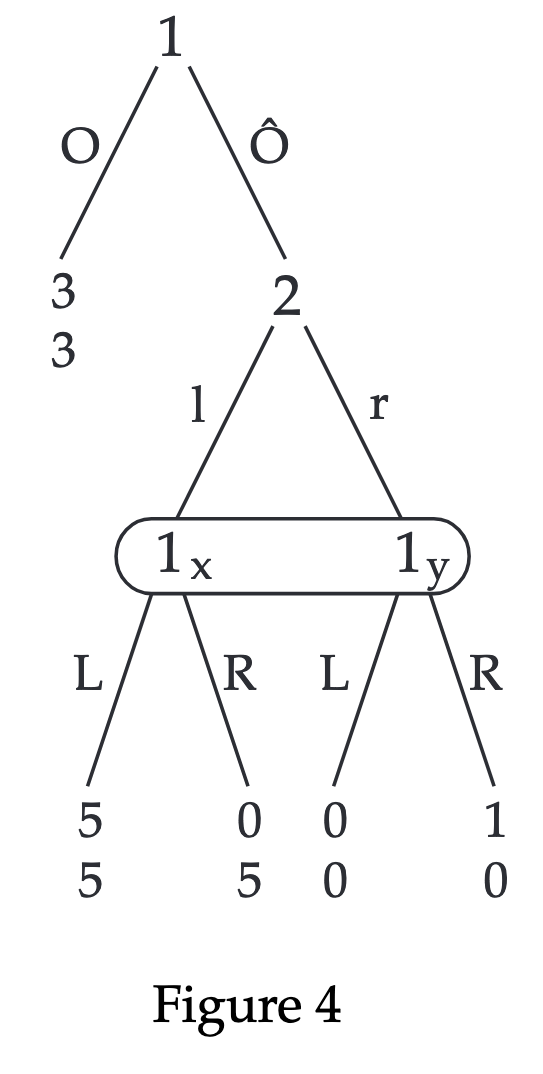
\includegraphics[width = 0.25\textwidth]{fig4.png}
  \end{center}
  \subsection*{Solution}
    $S = \{(\hat{O}, L), l\}$ is the strategy profile. The belief profile is such that $\mu_x \geq \frac{1}{4}, \ \mu_y < \frac{3}{4}$. 
\end{document}
